\documentclass[a4paper,twoside]{article}
\usepackage[T1]{fontenc}
\usepackage[bahasa]{babel}
\usepackage{graphicx}
\usepackage{graphics}
\usepackage{float}
\usepackage[cm]{fullpage}
\pagestyle{myheadings}
\usepackage{etoolbox}
\usepackage{setspace} 
\usepackage[dvipsnames]{xcolor}
\usepackage{lipsum} 
\usepackage{xspace}
\usepackage{hyperref}
\setlength{\headsep}{30pt}
\usepackage[inner=2cm,outer=2.5cm,top=2.5cm,bottom=2cm]{geometry} %margin
% \pagestyle{empty}

\hypersetup{colorlinks=true,urlcolor=SkyBlue,linkcolor=MidnightBlue}

\makeatletter
\renewcommand{\@maketitle} {\begin{center} {\LARGE \textbf{ \textsc{\@title}} \par} \bigskip {\large \textbf{\textsc{\@author}} }\end{center} }
\renewcommand{\thispagestyle}[1]{}
\markright{\textbf{\textsc{AIF184001/AIF184002 \textemdash Rencana Kerja Tugas Akhir \textemdash Sem. Genap 2024/2025}}}

\newcommand{\HRule}{\rule{\linewidth}{0.4mm}}
\newcommand{\web}{\textit{web}\xspace}
\renewcommand{\baselinestretch}{1}
\setlength{\parindent}{0 pt}
\setlength{\parskip}{6 pt}

\onehalfspacing

\begin{document}
	
	\title{\@judultopik}
	\author{\nama \textendash \@npm} 
	
	%tulis nama dan NPM anda di sini:
	\newcommand{\nama}{Alfonsus Oktario Sutomo}
	\newcommand{\@npm}{6181801010}
	\newcommand{\@judultopik}{Perkembangan Penggunaan Teknologi Pembangunan Web Dunia} % Judul/topik anda
	\newcommand{\jumpemb}{1} % Jumlah pembimbing, 1 atau 2
	\newcommand{\tanggal}{19/02/2025}
	
	% Dokumen hasil template ini harus dicetak bolak-balik !!!!
	
	\maketitle
	
	\pagenumbering{arabic}
	
	\section{Deskripsi}
	Internet merupakan jaringan yang menghubungkan berbagai macam perangkat yang memungkinkan pertukaran informasi secara cepat. Pertukaran informasi di internet diatur oleh sebuah protokol. Protokol tersebut adalah TCP/IP(\textit{Transmission Control Protocol/Internet Protocol}). Informasi yang diberikan oleh penyedia informasi tentunya harus mudah dimengerti oleh orang yang mengakses informasi tersebut. Informasi yang mudah dimengerti tidak hanya dalam bentuk tulisan, namun bisa juga berupa gambar, video, atau suara. Kebutuhan inilah yang menyebabkan munculnya layanan \web yang berjalan di atas internet.

    Layanan \web(\textit{World Wide Web}) memiliki protokol HTTP(\textit{HyperText Transfer Protocol}) sebagai aturan dalam pertukaran informasi yang dilakukan. Layanan \web ini dibangun dengan menggunakan berbagai teknologi yang ada, dalam perkembangannya banyak bermunculan pihak ketiga yang memberikan layanan berupa teknologi untuk membuat halaman web dari segi \textit{front end} maupun dari segi \textit{back end}, beberapa contoh dari teknologi tersebut adalah PHP, JavaScript, dan MySQL. Perkembangan teknologi ini kemudian dicatat oleh sebuah situs bernama \textit{HTTP Archive}.

    Situs \web \textit{HTTP archive} ini mencatat perkembangan teknologi yang dipakai dalam membuat \web. Situs ini mencatat perkembangan penggunaan teknologi berdasarkan beberapa kriteria seperti pengalaman pengguna dalam menggunakan \web, kecepatan sebuah \web dalam memuat informasi, dan tingkat aksesibilitas sebuah \web. Dalam penelitian ini aspek yang akan diamati dari perkembangan teknologi pembuatan \web adalah CrUX(\textit{Chrome User Experience}). Aspek ini mengukur tingkat interaktif dan lamanya sebuah \web dalam memuat informasi berdasarkan pengalaman nyata pengguna Chrome dengan kondisi yang bervariasi. 

    Data yang telah didapatkan dari situs \web \textit{HTTP archive} ini disimpan ke dalam sebuah layanan penyimpanan data berbasis \textit{cloud} yang dikembangkan oleh Google yaitu \textit{Google Big Query}. Layanan ini memungkinkan penggunanya untuk memproses data dengan menggunakan \textit{query SQL}. SQL sendiri merupakan bahasa pemrograman untuk mengelola \textit{big data}. SQL juga memiliki fungsi untuk menyimpan, mengubah, menghapus, dan mengambil data dalam sistem manajemen basis data.

        \begin{figure}[]
        \centering
        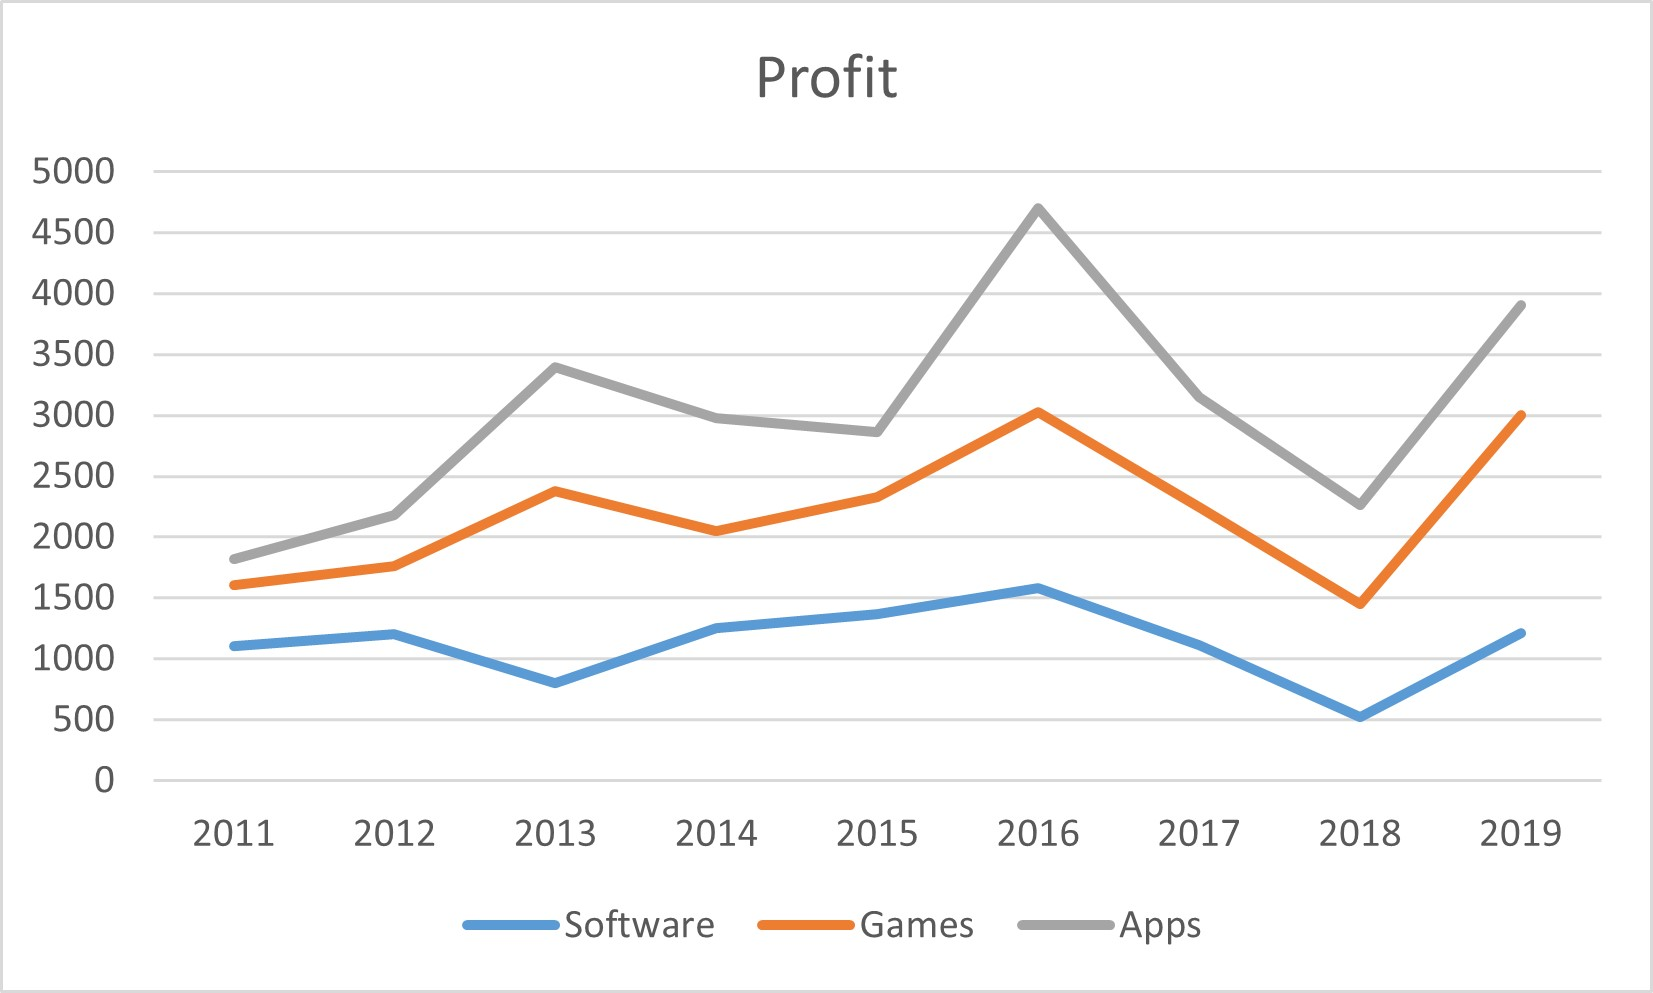
\includegraphics[width=0.5\linewidth]{Gambar/contoh linechart.jpg}
        \caption{Contoh \textit{line chart}}
        \label{fig:contohlinechart}
    \end{figure}

    Data perkembangan ini kemudian disajikan dalam bentuk visualisasi agar lebih mudah dimengerti. Salah satu bentuk visualisasi yang dapat digunakan untuk menjelaskan perkembangan ini adalah \textit{line chart}. Contoh \textit{line chart} dapat dilihat pada gambar~\ref{fig:contohlinechart}\footnote{Gambar didapatkan dari \url{https://www.simonsezit.com/article/how-to-make-a-line-graph-in-excel/}}. Visualisasi ini dapat memperlihatkan perkembangan secara jelas dengan rentang waktu yang lebih lebar. Hal ini berguna karena data yang digunakan adalah data dari 60 bulan terakhir atau data dari bulan oktober 2018 hingga bulan desember 2024.
	
	\section{Rumusan Masalah}
	Rumusan masalah yang akan diselesaikan dalam penelitian ini adalah:
    \begin{enumerate}
        \item Bagaimana perkembangan teknologi pembuatan \web selama 60 bulan terakhir?
        \item Bagaimana pekembangan teknologi pembuatan \web yang banyak digunakan oleh pembuat \web?
        \item Bagaimana cara menyajikan pekembangan teknologi pembuatan \web kepada pengguna?
    \end{enumerate}
	
	\section{Tujuan}
	Tujuan dari penelitian ini adalah:
    \begin{enumerate}
        \item Mengetahui perkembangan teknologi pembuatan \web selama 60 bulan terakhir.
        \item Mengetahui perkembangan teknologi pembuatan \web yang banyak digunakan oleh pembuat \web.
        \item Membuat perangkat lunak untuk menyajikan perkembangan teknologi pembuatan \web.
    \end{enumerate}
	
	\section{Deskripsi Perangkat Lunak}
	Perangkat lunak akhir yang akan dibuat memiliki fitur minimal sebagai berikut:
	\begin{itemize}
		\item Pengguna dapat melihat hasil perkembangan penggunaan teknologi pembuatan \web
		\item Pengguna dapat menentukan teknologi yang ingin dilihat  
		\item Pengguna dapat mengatur rentang waktu data yang ingin dilihat
		\item Pengguna dapat mengatur jenis data yang ingin dilihat dapat berdasarkan jumlah atau persentase dari teknologi yang digunakan
	\end{itemize}
	
	\section{Detail Pengerjaan Tugas Akhir}
	Bagian-bagian pekerjaan skripsi ini adalah sebagai berikut :
	\begin{enumerate}
		\item Melakukan studi literatur mengenai teknologi pembuatan \web
		\item Melakukan studi literatur mengenai bahasa SQL
            \item Melakukan studi literatur mengenai statistika
		\item Melakukan studi literatur mengenai visualisasi data
		\item Mempelajari penggunaan \textit{Google Big Query}
		\item Melakukan pengumpulan data perkembangan teknologi pembuatan \web
		\item Melakukan analisa dan visualisasi terhadap data perkembangan teknologi pembuatan \web
		\item Membangun GUI yang menampilkan hasil analisis dengan fitur yang interaktif 
		\item Menulis dokumen tugas akhir.
	\end{enumerate}
	
	\section{Rencana Kerja}
	Rincian capaian yang direncanakan di Tugas Akhir 1 adalah sebagai berikut:
	\begin{enumerate}
            \item Melakukan studi literatur mengenai teknologi pembuatan \web
		\item Melakukan studi literatur mengenai bahasa SQL
            \item Melakukan studi literatur mengenai statistika
		\item Melakukan studi literatur mengenai visualisasi data
		\item Mempelajari penggunaan \textit{Google Big Query}
            \item Menulis dokumen tugas akhir
	\end{enumerate}
	
	Sedangkan yang akan diselesaikan di Tugas Akhir 2 adalah sebagai berikut:
	\begin{enumerate}
            \item Melakukan pengumpulan data perkembangan teknologi pembuatan \web
		\item Melakukan analisa dan visualisasi terhadap data perkembangan teknologi pembuatan \web
		\item Membangun GUI yang menampilkan hasil analisis dengan fitur yang interaktif 
		\item Menulis dokumen tugas akhir.
	\end{enumerate}
	
	\vspace{1cm}
	\centering Bandung, \tanggal\\
	\vspace{2cm} \nama \\ 
	\vspace{1cm}
	
	Menyetujui, \\
	\ifdefstring{\jumpemb}{2}{
		\vspace{1.5cm}
		\begin{centering} Menyetujui,\\ \end{centering} \vspace{0.75cm}
		\begin{minipage}[b]{0.45\linewidth}
			% \centering Bandung, \makebox[0.5cm]{\hrulefill}/\makebox[0.5cm]{\hrulefill}/2013 \\
			\vspace{2cm} Nama: \makebox[3cm]{\hrulefill}\\ Pembimbing Utama
		\end{minipage} \hspace{0.5cm}
		\begin{minipage}[b]{0.45\linewidth}
			% \centering Bandung, \makebox[0.5cm]{\hrulefill}/\makebox[0.5cm]{\hrulefill}/2013\\
			\vspace{2cm} Nama: \makebox[3cm]{\hrulefill}\\ Pembimbing Pendamping
		\end{minipage}
		\vspace{0.5cm}
	}{
		% \centering Bandung, \makebox[0.5cm]{\hrulefill}/\makebox[0.5cm]{\hrulefill}/2013\\
		\vspace{2cm} Pascal~Alfadian,~Nugroho,~M.Comp.\\ Pembimbing Tunggal
	}
\end{document}
